\chapter{Dashboard}
\label{cha:dashboard}

Das Dashboard bietet Überblicke und Statistiken. Ist ein Benutzer mehreren Gliederungen zugewiesen, wird auf dem Dashboard nur Inhalte der aktuell ausgewählten Gliederung dargestellt.

\begin{itemize}
\item Geleistete Dienste: Summe der Dienste aus der aktueller Saison, bei welchem der Benutzer eine Position übernommen hatte.
\item Total Geleistete Dienste: Summe der Positionen welche in der aktuellen Saison von allen geleistet wurde.
\item Noch nicht besetzte Dienste: Summe der zukünftig noch nicht besetzten Positionen. Hier werden nur Positionen welche für eine Mindestbesatzung relevant sind aufgezählt.
\item Hall of Fame: Benutzer mit den am meisten geleisteten Diensten der aktuellen Saison. 
\end{itemize}

\noindent Darunter sind News (Kapitel \ref{cha:nachrichten}) wie auch neue Infos zu finden. Diese werden meist ebenfalls per E-Mail den Benutzern zugestellt.

\begin{figure}[h]
 \begin{addmargin}{-0.2\linewidth}
   \centering 
   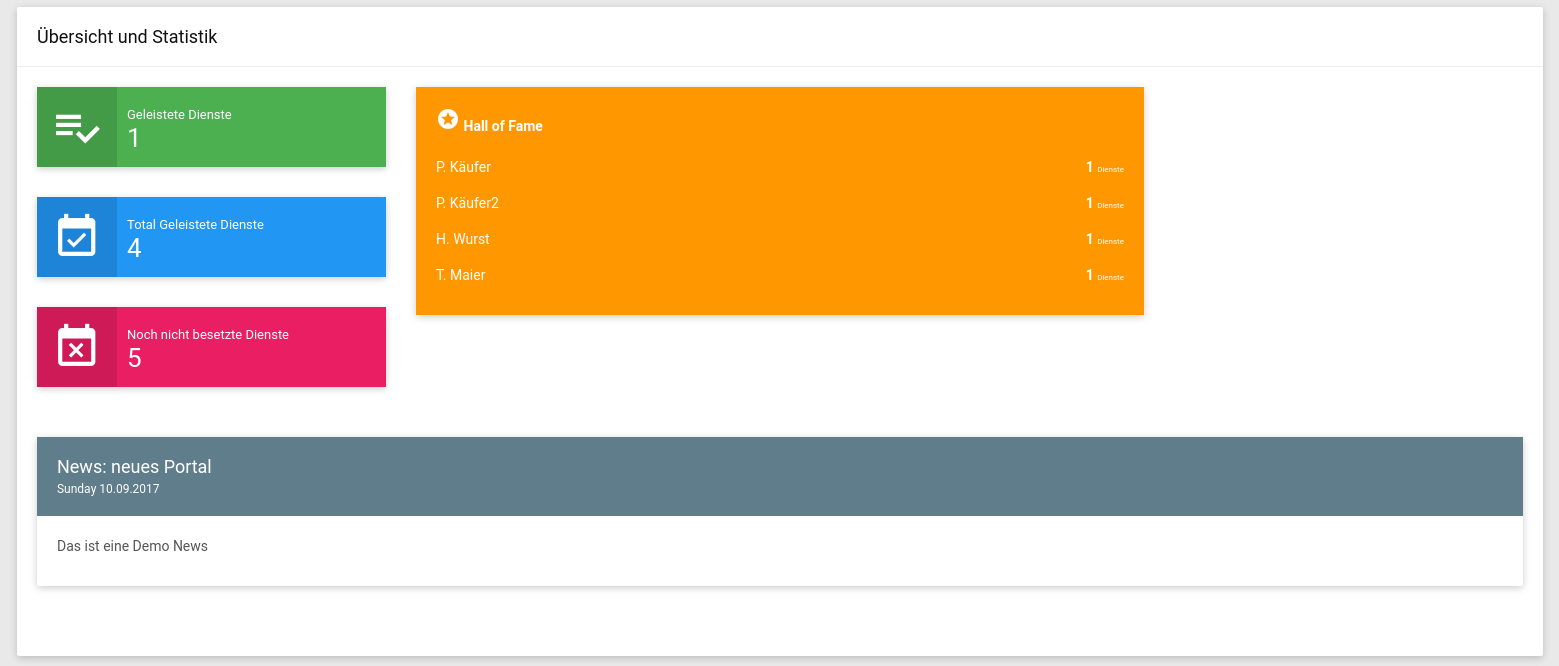
\includegraphics[width=20cm]{Bilder/view_overview.png}
 \end{addmargin} 
 \caption[Dashboard ansicht]{DLRG Dienstplan Dashboard ansicht}
 \label{fig:view_overview}
\end{figure}